\documentclass[11pt,a4paper]{article}
\newcommand{\simname}{Cylinder Shot Peening Coverage Simulator}
\usepackage[utf8]{inputenc}
\usepackage[T1]{fontenc}
\usepackage[sc]{mathpazo}
\linespread{1.05}
\usepackage[english]{babel}
\usepackage[margin=2.2cm]{geometry}
\usepackage{amsmath,amssymb}
\usepackage[locale=UK,per-mode=symbol]{siunitx}
\usepackage{booktabs,array,tabularx,longtable}
\usepackage{graphicx}
\usepackage{tikz}
\usetikzlibrary{arrows.meta,decorations.pathreplacing,calc}
\usepackage{xcolor}
\usepackage[hidelinks]{hyperref}
\usepackage{enumitem}
\usepackage{tcolorbox}
\usepackage{float}
\usepackage[font=small,labelfont=bf]{caption}
\usepackage{subcaption}
\usepackage{fancyhdr}
\usepackage{multicol}

\definecolor{bleu}{HTML}{1F5A96}
\definecolor{orange}{HTML}{D4621C}
\definecolor{vert}{HTML}{2E8B57}
\definecolor{rouge}{HTML}{E5484D}
\newtcolorbox{keybox}[1][]{colback=bleu!5,colframe=bleu,boxrule=0.6pt,arc=2pt,left=6pt,right=6pt,top=4pt,bottom=4pt,#1}
\newtcolorbox{trybox}[1][]{colback=orange!6,colframe=orange,boxrule=0.6pt,arc=2pt,left=6pt,right=6pt,top=4pt,bottom=4pt,#1}
\newcommand{\E}{\mathbb{E}}
\newcommand{\dX}{\Delta X}
\newcommand{\ui}[1]{\textsf{#1}}   % name of a control or a readout on the page
\setlength{\tabcolsep}{5pt}
\renewcommand{\arraystretch}{1.15}

\pagestyle{fancy}
\fancyhf{}
\fancyhead[L]{\small Dr Régis Kubler, Arts et Métiers Institute of Technology}
\fancyhead[R]{\small\simname}
\fancyfoot[C]{\small\thepage}
\renewcommand{\headrulewidth}{0.4pt}
\setlength{\headheight}{14pt}
\setlength{\parskip}{3pt}
\usepackage{newunicodechar}
\newunicodechar{λ}{\ensuremath{\lambda}}
\newunicodechar{Σ}{\ensuremath{\Sigma}}
\newunicodechar{Δ}{\ensuremath{\Delta}}
\newunicodechar{δ}{\ensuremath{\delta}}
\newunicodechar{τ}{\ensuremath{\tau}}
\newunicodechar{σ}{\ensuremath{\sigma}}
\newunicodechar{η}{\ensuremath{\eta}}
\newunicodechar{α}{\ensuremath{\alpha}}
\newunicodechar{φ}{\ensuremath{\varphi}}
\newunicodechar{ζ}{\ensuremath{\zeta}}
\newunicodechar{²}{\ensuremath{^2}}
\newunicodechar{³}{\ensuremath{^3}}
\newunicodechar{−}{\ensuremath{-}}
\newunicodechar{·}{\ensuremath{\cdot}}
\newunicodechar{×}{\ensuremath{\times}}
\newunicodechar{≈}{\ensuremath{\approx}}
\newunicodechar{≥}{\ensuremath{\geq}}
\newunicodechar{≤}{\ensuremath{\leq}}
\newunicodechar{→}{\ensuremath{\rightarrow}}
\newunicodechar{°}{\ensuremath{^\circ}}
\newunicodechar{µ}{\ensuremath{\mu}}
\newunicodechar{…}{\ldots}
\newunicodechar{ṁ}{\ensuremath{\dot m}}
\newunicodechar{Ṅ}{\ensuremath{\dot N}}
\newunicodechar{₀}{\ensuremath{_0}}
\newunicodechar{₉}{\ensuremath{_9}}
\newunicodechar{₈}{\ensuremath{_8}}
\newunicodechar{₅}{\ensuremath{_5}}


\title{\textbf{Cylinder Shot Peening Coverage Simulator}\\[3pt]
\large User and theory guide: coverage of a rotating cylinder and helical stripes}
\author{Dr Régis Kubler\\ Arts et Métiers Institute of Technology\\[4pt]
\small Developed with the assistance of Claude Opus 5.5 (Anthropic), November 2026}
\date{Guide for simulator version 1.5 (18 November 2026)\\ \url{https://rkubler.github.io/cylinder-coverage/}}

\begin{document}
\maketitle
\thispagestyle{fancy}

\begin{abstract}
\noindent This guide explains the Cylinder Shot Peening Coverage Simulator. A cylinder turns while the nozzle travels along its axis, so the jet draws a helix on the surface. The guide starts with the basic idea and a first experiment, then explains the helix, the average and helical stripe models, the curvature of the surface, back-and-forth and one-way passes, every parameter, every result and chart displayed, the specified coverages above 100\,\% (treatment times) of NF~L~06-832, the algorithm and its validation.
\end{abstract}

\tableofcontents

\section{The idea in one page}

\paragraph{A helix on a turning part.} Shafts, pins and springs are often peened while they turn on centres. The cylinder of radius $R$ turns at $N$ revolutions per minute, and the nozzle, aimed at the axis, travels along it at the traverse speed $V$. Seen from the surface, the jet moves around the cylinder and slowly along it: it draws a \emph{helix}. During one turn the nozzle advances by the \emph{pitch}
\begin{equation}
\boxed{p=\frac{60\,V}{N}}\qquad(V\text{ in mm/s},\ N\text{ in rpm}).
\end{equation}
If the pitch is small compared with the jet size $\dX$, successive turns overlap a lot and the surface is treated evenly. If the pitch is large, the impacts pile up along the helix and leave weaker bands between its turns: \emph{helical stripes}.

\paragraph{What the page computes.} For each point of the surface it computes the expected number of impacts $\lambda$ and the local coverage $\tau=1-e^{-\lambda}$, shows the rotating cylinder and the unrolled surface, and compares the mean coverage with an \textbf{average model} (impacts spread evenly) and a \textbf{helical stripe model} (stripes taken into account).

\begin{figure}[H]
\centering
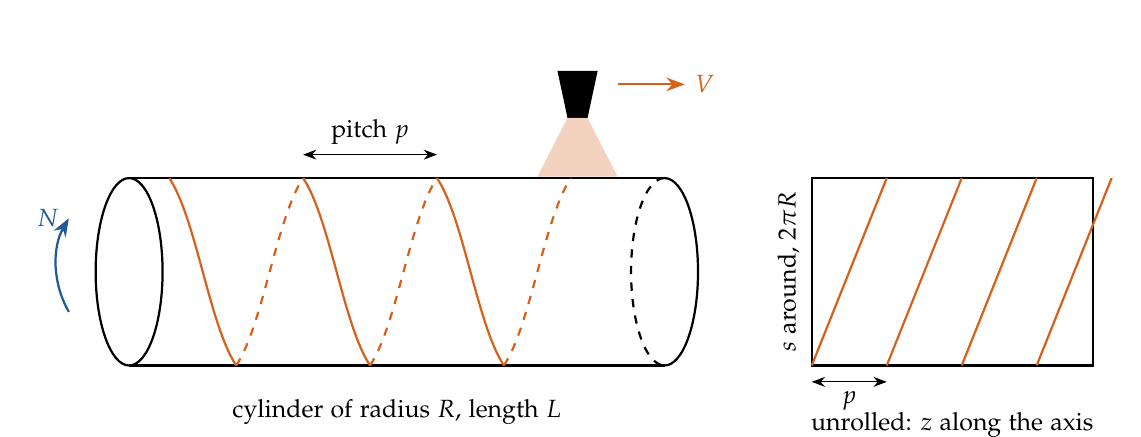
\begin{tikzpicture}[scale=0.85,>=Stealth]
% cylinder
\draw[thick] (0,0) ellipse (0.5 and 1.4);
\draw[thick] (0,1.4) -- (8,1.4); \draw[thick] (0,-1.4) -- (8,-1.4);
\draw[thick] (8,1.4) arc (90:-90:0.5 and 1.4);
\draw[thick,dashed] (8,1.4) arc (90:270:0.5 and 1.4);
\foreach \x in {0.6,2.6,4.6} { \draw[orange,thick] (\x,1.4) .. controls (\x+0.4,0.8) and (\x+0.6,-0.8) .. (\x+1,-1.4); \draw[orange,thick,dashed] (\x+1,-1.4) .. controls (\x+1.4,-0.8) and (\x+1.6,0.8) .. (\x+2,1.4); }
\draw[<->] (2.6,1.75) -- (4.6,1.75) node[midway,above] {\small pitch $p$};
% nozzle
\fill[black] (6.4,3.0) -- (7.0,3.0) -- (6.85,2.3) -- (6.55,2.3) -- cycle;
\fill[orange!35,opacity=.8] (6.55,2.3) -- (6.85,2.3) -- (7.3,1.42) -- (6.1,1.42) -- cycle;
\draw[->,thick,orange] (7.3,2.8) -- (8.3,2.8) node[right] {\small $V$};
\draw[->,thick,bleu] (-0.9,-0.6) arc (210:150:1.4) node[left] {\small $N$};
\node[font=\small] at (4,-2.1) {cylinder of radius $R$, length $L$};
% unrolled
\begin{scope}[xshift=10.2cm,yshift=-1.4cm,scale=0.7]
\draw[thick] (0,0) rectangle (6,4);
\foreach \x in {0,1.6,3.2,4.8} \draw[orange,thick] (\x,0) -- (\x+1.6,4);
\draw[<->] (0,-0.35) -- (1.6,-0.35) node[midway,below] {\small $p$};
\node[font=\small,below] at (3,-0.8) {unrolled: $z$ along the axis};
\node[font=\small,rotate=90] at (-0.5,2) {$s$ around, $2\pi R$};
\end{scope}
\end{tikzpicture}
\caption{The jet draws a helix of pitch $p$ on the turning cylinder. Unrolled, the helix becomes a set of parallel straight lines, tilted by the helix angle $\alpha$.}
\label{fig:helix}
\end{figure}

\begin{trybox}
\textbf{First experiment.} The page opens with the reference media and jet ($\dot m=\SI{1.5}{kg/min}$, glass beads, $D=\SI{150}{\micro m}$, $r=\SI{10}{\micro m}$, Gaussian jet $\dX=\SI{20}{mm}$), a cylinder of radius \SI{25}{mm} and length \SI{150}{mm} turning at 24\,rpm, and a traverse speed of \SI{8}{mm/s}. Then:
\begin{itemize}[nosep]
\item the surface moves at $V_s=\SI{62.8}{mm/s}$ and the pitch is $p=\SI{20}{mm}$, as large as the jet: the helix is clearly visible;
\item after 2 passes back and forth, the mean coverage is \SI{94.0}{\percent}, between \SI{76.1}{\percent} and \SI{99.4}{\percent}; the average model says \SI{96.0}{\percent};
\item 98\,\% needs 2.6 passes, full coverage (NF~L~06-832) 3.3 passes.
\end{itemize}
Now set $N=48$\,rpm: the pitch falls to \SI{10}{mm}, the stripes drop from 114\,\% to 2.8\,\%, and the mean coverage rises to \SI{96.0}{\percent} for the same time.
\end{trybox}

\section{The screen}

\begin{figure}[H]
\centering
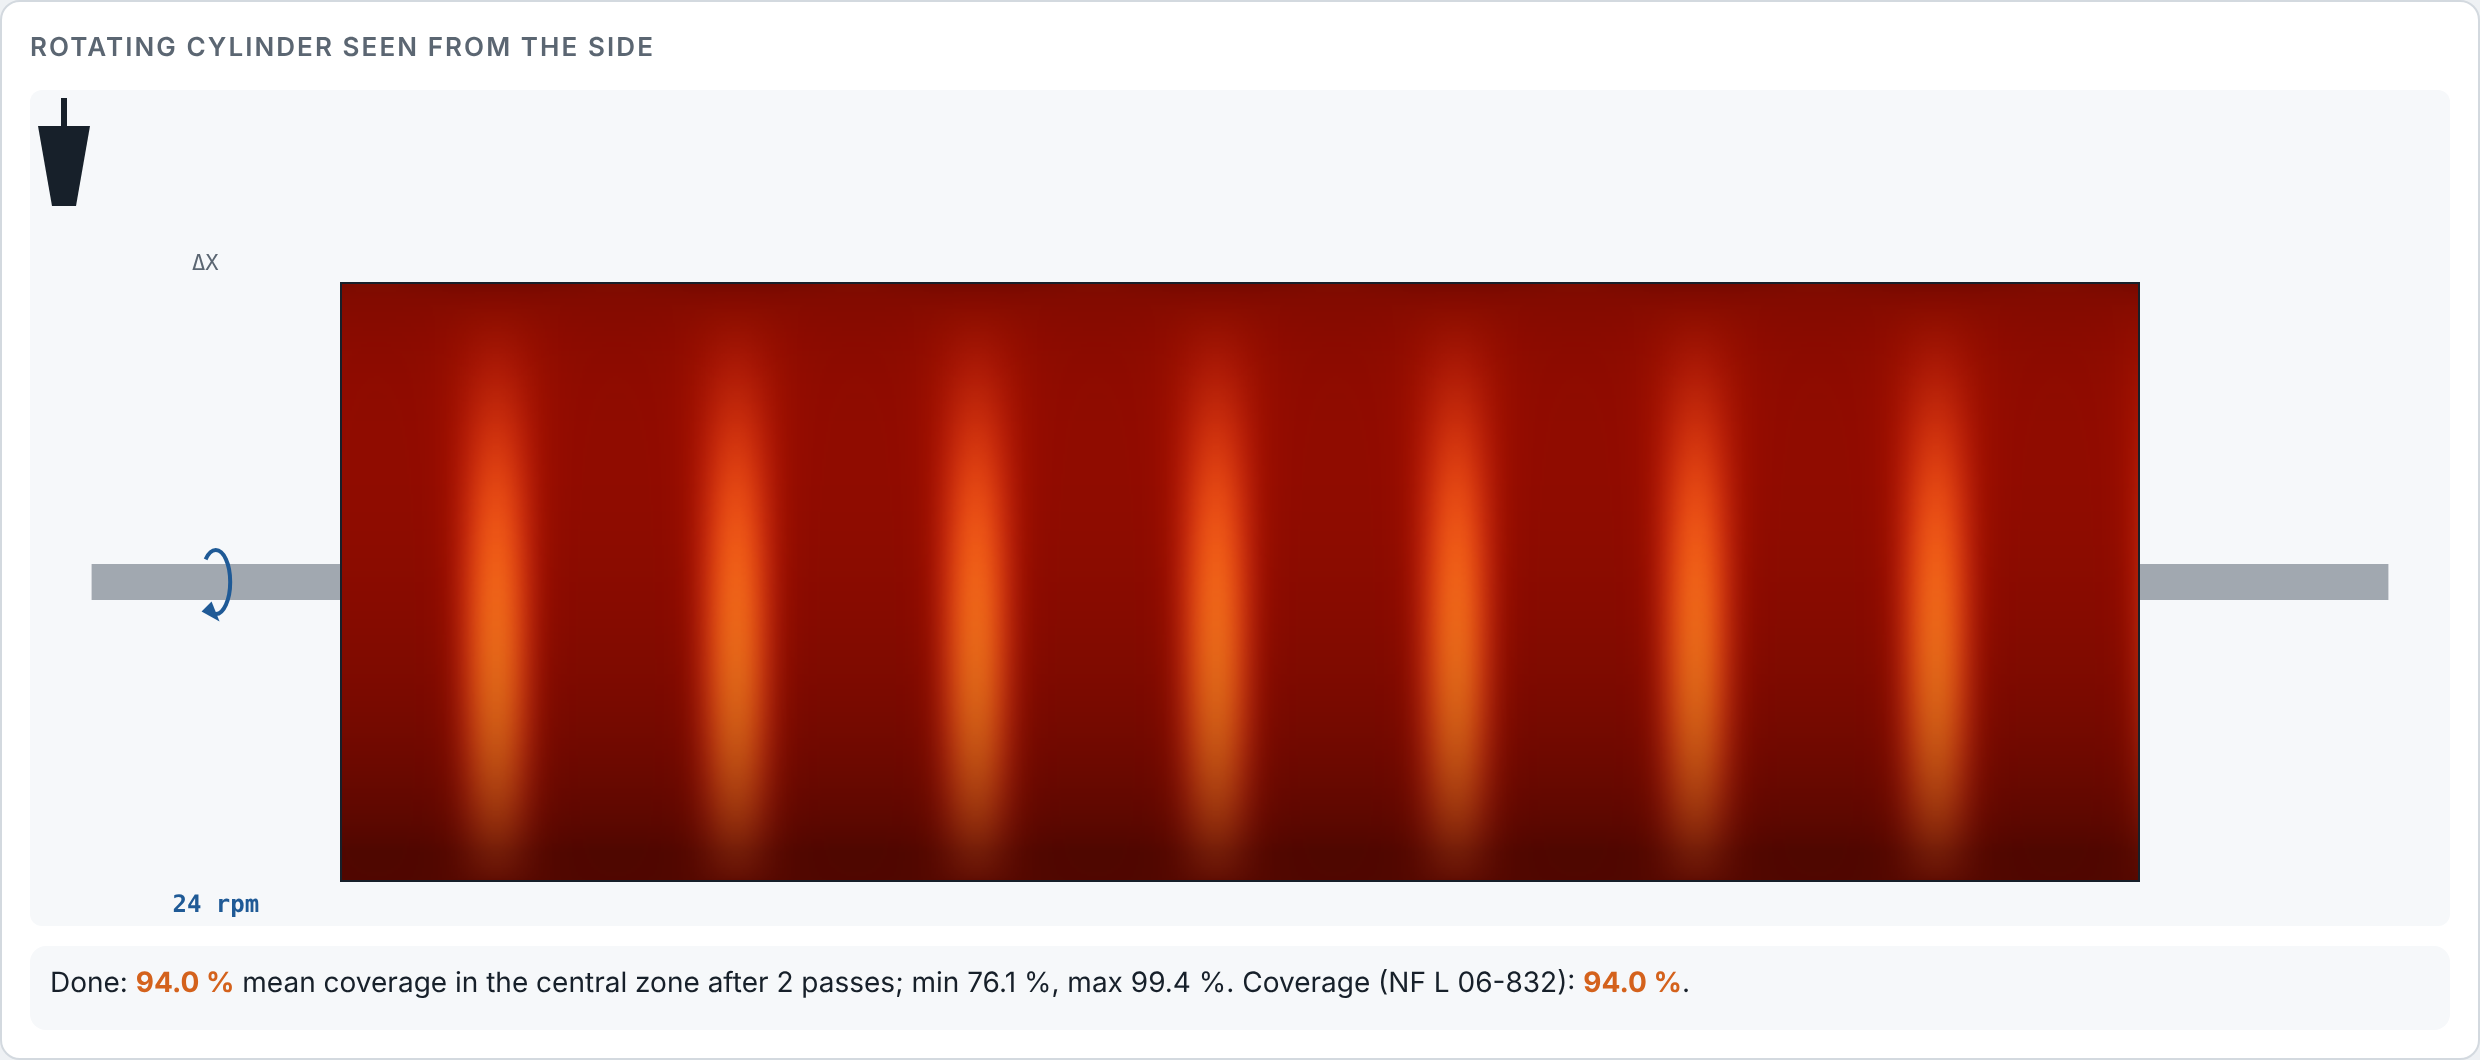
\includegraphics[width=\linewidth]{img/sec0.png}
\caption{Rotating cylinder seen from the side: the nozzle (top), the jet hitting the top of the cylinder, the traverse direction and the rotation speed. The surface turns towards the viewer, so the treated band rolls down the visible face.}
\end{figure}

\paragraph{Toolbar.}
\begin{description}[leftmargin=2.6cm,style=nextline,itemsep=2pt]
\item[\ui{Play / Pause}] runs or stops the animation.
\item[\ui{+1 turn}] plays one revolution of the cylinder and stops.
\item[\ui{+1 pass}] completes the current pass (one traverse along the axis) and stops.
\item[\ui{Run all}] computes all the passes at once.
\item[\ui{Restart}] clears the surface (and draws new random phases if that option is chosen).
\item[\ui{Time}] \ui{auto} plays one pass in about 10 seconds whatever the settings; \ui{real time} plays at the real process speed; $\times3$ to $\times1000$ accelerate it.
\item[\ui{Maps show}] coverage $\tau$, impacts per point $\lambda$, or local coverage (NF~L~06-832), which can exceed 100\,\%, on both the 3D view and the unrolled map.
\end{description}

\paragraph{Panels.}
\begin{enumerate}[nosep]
\item \textbf{Rotating cylinder seen from the side}, with a status line below it.
\item \textbf{Unrolled surface}: axial position $z$ across, circumferential position $s$ down (from 0 to $2\pi R$). The dashed lines show the path of the current pass, the orange rectangle the jet footprint, the vertical dashed lines the limits of the central zone used for statistics. When the circumference is much longer or shorter than the cylinder, the vertical axis is compressed or stretched, and a note says so. Hovering gives $z$, $s$, the angle, $\lambda$, $\tau$ and the local coverage (NF~L~06-832); clicking moves the cross-section.
\item \textbf{Cross-section along the axis} at the chosen $s$: $\tau(z)$ (orange) and $\lambda(z)$ (blue), with the crossings of the last helix as dotted marks, and the main readouts.
\item \textbf{Coverage versus number of passes}, with the time readouts.
\item \textbf{One-pass coverage versus rotation speed} from 1 to 60\,rpm.
\item \textbf{Parameters} and \textbf{How the cylinder model works} (calculation chain).
\end{enumerate}

\begin{figure}[H]
\centering
\begin{subfigure}{0.49\linewidth}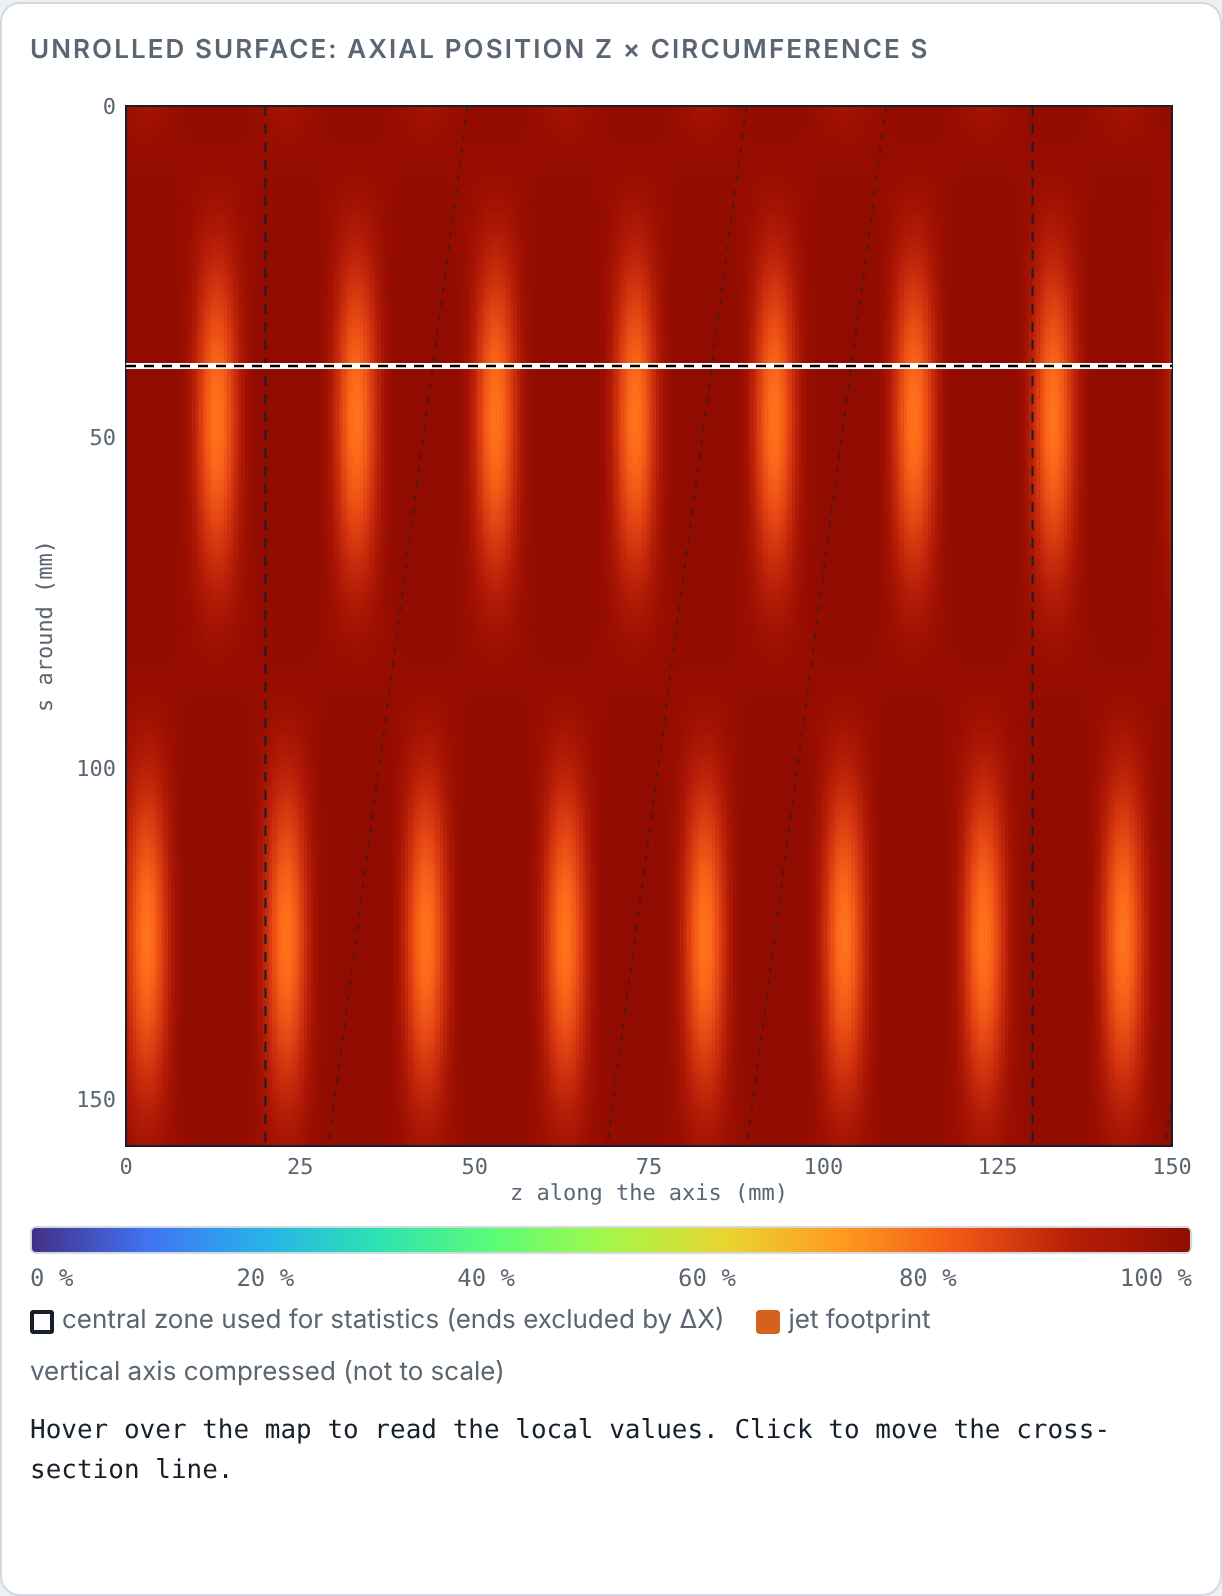
\includegraphics[width=\linewidth]{img/sec1.png}\caption{Unrolled surface}\end{subfigure}\hfill
\begin{subfigure}{0.49\linewidth}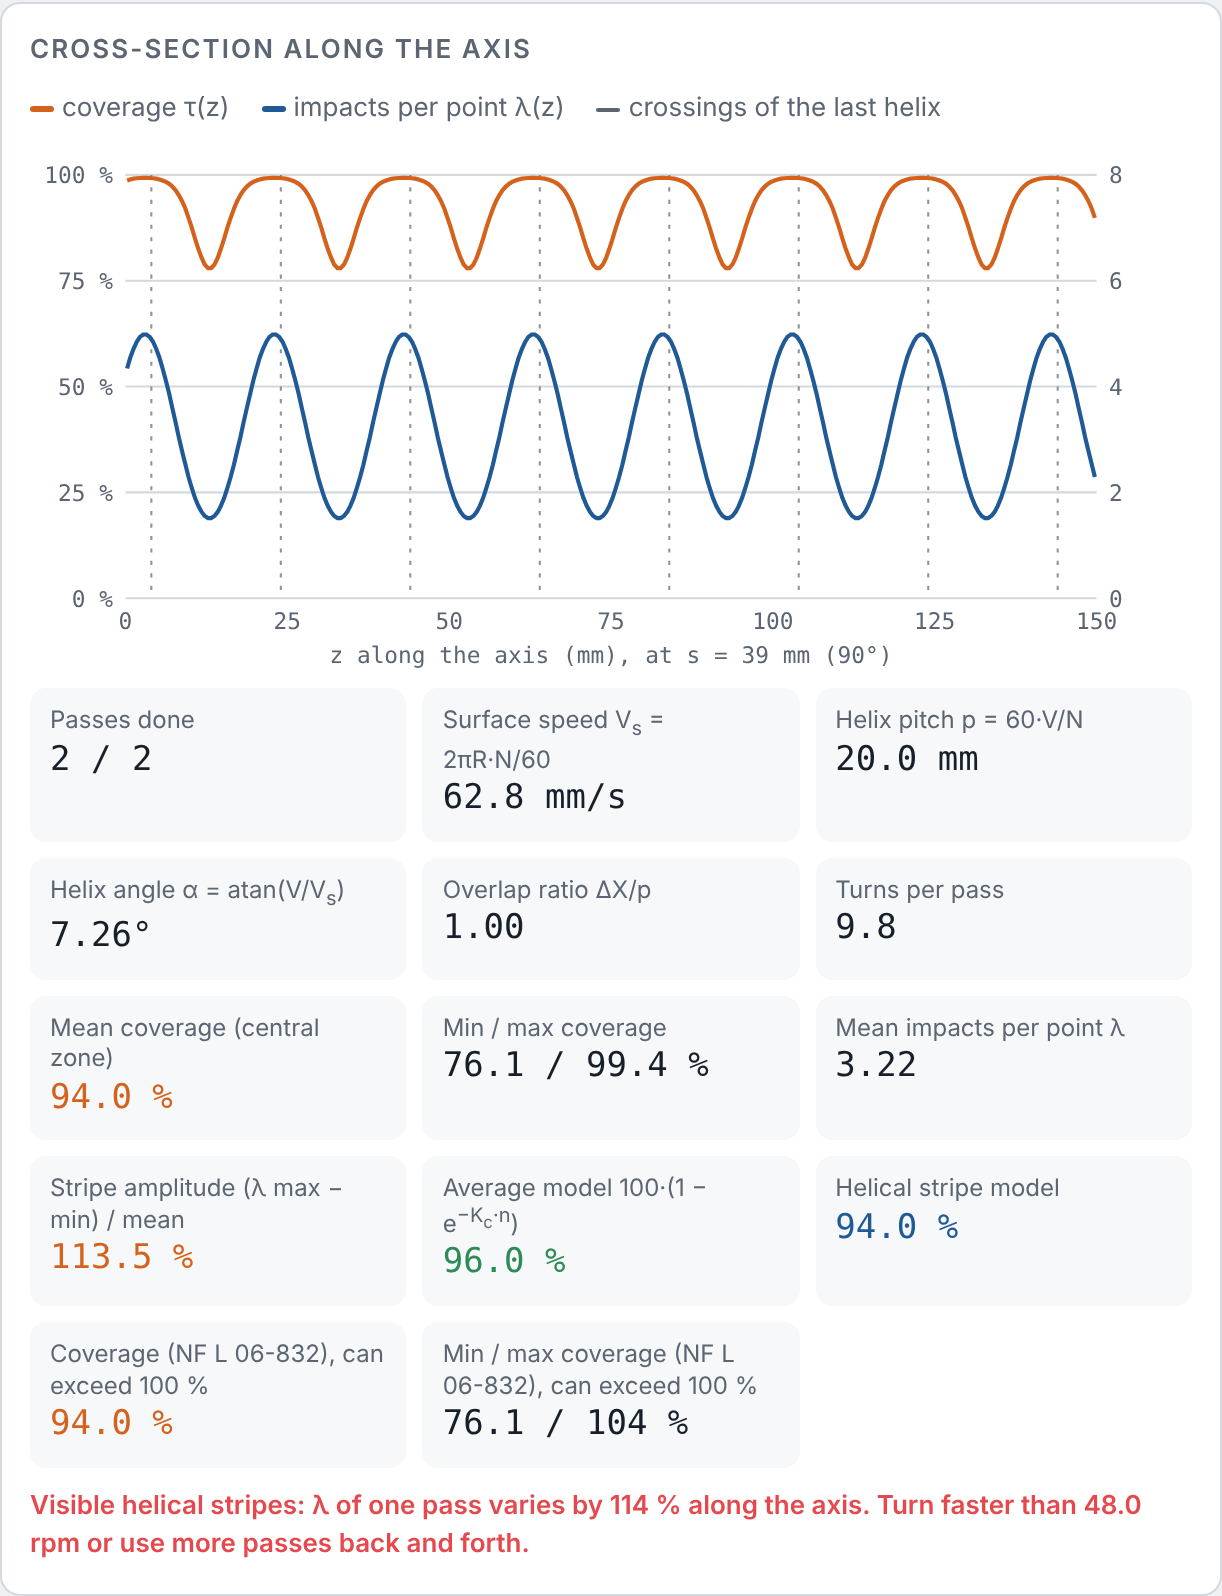
\includegraphics[width=\linewidth]{img/sec2.png}\caption{Cross-section and readouts}\end{subfigure}
\caption{After 2 passes back and forth with the defaults: the two helices of opposite hands cross and leave a diamond pattern.}
\end{figure}

\section{Kinematics of the helix}

\begin{align}
V_s&=\frac{2\pi R\,N}{60} && \text{surface speed [\SI{62.8}{mm/s}]},\\
p&=\frac{60\,V}{N}=2\pi R\,\frac{V}{V_s} && \text{pitch, axial advance per turn [\SI{20}{mm}]},\\
\alpha&=\arctan\frac{V}{V_s} && \text{helix angle [7.26°]}.
\end{align}
Relative to the surface the nozzle moves with the velocity $(V,V_s)$: along the axis at $V$ and around at $V_s$. Unrolled, the path is a set of straight lines tilted by $\alpha$, spaced by $p$ along the axis (Fig.~\ref{fig:helix}). The overlap ratio $\dX/p$ [1.00] plays the role of $\dX/\delta$ for a flat raster.

A \textbf{pass} is one traverse along the axis, from an overtravel before the cylinder to an overtravel after it. Each overtravel equals the reach of the jet plus 2\,\% of the length, so that the ends of the cylinder are treated like its middle:
\begin{equation}
T_p=\frac{L+2\,o_v}{V}\ [\SI{24.5}{s}],\qquad\text{turns per pass}=\frac{T_p\,N}{60}\ [9.8].
\end{equation}

\section{Average model}

One pass throws $\dot N\,T$ shots in the time $T=L/V$ that the nozzle needs to cross the cylinder, and spreads them over the area $2\pi R\,L$. The mean number of impacts per point and per pass is therefore
\begin{equation}
\boxed{K_c=\frac{c\,a\,\dot N}{2\pi R\,V}}\quad[1.608],
\end{equation}
where $a$ is the mean dent area, $\dot N$ the number of shots per second (see the local coverage guide) and $c$ the fraction of the shots that hit the cylinder (Section~\ref{sec:curv}). The average model is
\begin{equation}
\tau_{\text{avg}}=100\,\bigl(1-e^{-K_c\,n}\bigr),\qquad n_{98,\text{avg}}=\frac{\ln 50}{K_c}.
\end{equation}
\begin{keybox}
\textbf{$K_c$ does not depend on the rotation speed.} Turning faster spreads the same shots over the same area; it only makes the helix finer. Equivalently, $K_c=c\,a\dot N/(V_s\,p)$: the cylinder behaves like a flat raster of step $p$ swept at the speed $V_s$. Compared with one pass along a single line of a flat part at the same speed $V$, $K_c=c\,K\,\dX/(2\pi R)$.
\end{keybox}

\section{Curvature of the surface}\label{sec:curv}

The jet is a parallel stream of width $\dX$ aimed at the axis. A shot that travels at a distance $u$ from the plane containing the axis hits the surface at the arc length
\begin{equation}
s=R\,\arcsin\frac{u}{R},
\end{equation}
and shots with $|u|>R$ miss the cylinder. A band $\mathrm{d}u$ of the jet spreads over the arc $\mathrm{d}s=\mathrm{d}u/\cos(s/R)$, so the density of shots per unit arc around the cylinder is
\begin{equation}
g_s(s)=g\!\left(R\sin\frac{s}{R}\right)\cos\frac{s}{R},\qquad |s|<\frac{\pi R}{2},
\end{equation}
where $g$ is the jet profile. The fraction of the shots that hit is $c=G(R)-G(-R)$, with $G$ the cumulative of $g$ [100\,\% for $R=\SI{25}{mm}$; 68.3\,\% for $R=\SI{5}{mm}$ with a \SI{20}{mm} Gaussian jet]. With the option \ui{Curvature ignored}, the surface is treated as flat: $g_s=g$ and $c=1$. That option is only meaningful when $\dX\ll R$; the page warns when the jet is wider than the cylinder. The incidence becomes oblique towards the edges of the footprint, which in reality makes the dents slightly smaller; this is not modelled.

\section{Helical stripes}

\paragraph{The helical coordinate.} Along the helix, every turn of the path is the same line shifted by $p$. The natural coordinate is
\begin{equation}
\zeta_+=z-s\,\frac{p}{2\pi R}\quad\text{(forward pass)},\qquad \zeta_-=z+s\,\frac{p}{2\pi R}\quad\text{(return pass)},
\end{equation}
which is constant along each helix. The impacts of one pass depend only on $\zeta$ and repeat with the period $p$:
\begin{equation}
\lambda_1(\zeta)=a\dot N\sum_k h(\zeta-k\,p),\qquad
h(\zeta)=\frac{1}{V_s}\int g(\zeta-\sigma\tan\alpha)\,g_s(\sigma)\,\mathrm{d}\sigma.
\label{eq:h}
\end{equation}
$h$ is the \emph{track profile}: the impacts received at an axial distance $\zeta$ from the passage of the jet, integrated over the time the footprint takes to cross the point. Its integral is $c/V_s$, which gives back $K_c$ for the mean.

\paragraph{Stripe amplitude.} The page gives $(\lambda_{\max}-\lambda_{\min})/\bar\lambda$ for one pass [114\,\%]. For a Gaussian jet with $\sigma_j=\dX/4$ and a small helix angle, the result of the flat raster applies with $\delta=p$:
\begin{equation}
\frac{\lambda_{\max}-\lambda_{\min}}{\bar\lambda}\simeq4\,e^{-2\pi^2(\sigma_j/p)^2},
\end{equation}
which is below 3\,\% for $p\le\dX/2$, that is
\begin{equation}
\boxed{N\ge\frac{120\,V}{\dX}}\quad[\text{48 rpm}].
\end{equation}
For the uniform jet the stripes vanish when $\dX/p$ is a whole number (for instance $p=\dX$: 0.3\,\% with the defaults); for the flattened Gaussian they are computed numerically.

\paragraph{Helical stripe model.} The mean coverage is the mean of $1-e^{-\lambda}$ over one period of the stripes. The page evaluates $\lambda_1$ on 256 points per period.

\section{Several passes}

\paragraph{Back and forth.} A return pass draws a helix of the opposite hand. The two families of stripes cross, and $\lambda=\Lambda_+(\zeta_+)+\Lambda_-(\zeta_-)$, where $\Lambda_\pm$ add up the forward and return passes. Over the surface $\zeta_+$ and $\zeta_-$ vary independently, so the mean coverage factorises:
\begin{equation}
\bar\tau=1-\bigl\langle e^{-\Lambda_+}\bigr\rangle\,\bigl\langle e^{-\Lambda_-}\bigr\rangle .
\end{equation}
As for crossed rasters on a flat part, crossing spreads the weak stripes of one family over the strong stripes of the other.

\paragraph{Same direction.} With \ui{Same direction, return with the jet off}, the nozzle comes back without peening (the return takes the same time as a pass) and every pass draws a helix of the same hand. The helices stack, shifted by a \emph{phase}
\begin{equation}
\varphi_i=\Bigl(z_{0,i}-s_{0,i}\,\frac{p}{2\pi R}\Bigr)\bmod p,
\end{equation}
where $z_{0,i}$ and $s_{0,i}$ are the axial and circumferential positions of the nozzle at the start of pass $i$. If the phases line up, the stripes add up; if they are spread, they fill each other.

\paragraph{Rotation angle at the start of a pass.} \ui{Follows from the motion}: the cylinder keeps turning during the whole process, so $s_{0,i}=V_s\,t_i$; the phases are deterministic. \ui{Random at each pass}: each pass starts at a random angle, as when the timing between passes is not controlled; \ui{Restart} draws new angles. The model uses the same phases as the simulation, so the two always agree.

\section{Coverage above 100\,\% (NF~L~06-832)}\label{sec:above}

The base time $t_b$ is the time to reach 98\,\% coverage, full coverage (100\,\%) is $1.25\,t_b$, and a coverage of $C$\,\% is $\frac{C}{100}\times1.25\,t_b$. On the page the base time comes from the helical stripe model ($n_{98}$ passes), full coverage needs $1.25\,n_{98}$ passes and the specified coverage $\frac{C}{100}\times1.25\,n_{98}$. On an even treatment, full coverage corresponds to $\lambda_{100}=1.25\ln50=4.89$ impacts per point (99.25\,\% dented). The option \ui{= base time} drops the factor 1.25 ($\lambda_{100}=3.91$, 98\,\% dented). A fraction of a pass stands for one pass with the same dose at a proportionally slower traverse speed; strictly, that would also make the helix finer, so it is an approximation.

\paragraph{The readout \ui{Coverage (NF L 06-832)}.} Coverage is the dented area divided by the total area as long as it can be measured, i.e.\ up to 98\,\%. Beyond, NF~L~06-832 counts time. The page combines both in one value, $C(t)$, continuous and increasing:
\begin{equation}
C(t)=\begin{cases}
\text{dented area (\%)} & t\le t_b\quad(\text{reaches }98\,\%\text{ at }t_b)\\[2pt]
98+2\,\dfrac{t/t_b-1}{0.25} & t_b<t\le1.25\,t_b\quad(98\to100\,\%)\\[6pt]
100\,\dfrac{t}{1.25\,t_b} & t>1.25\,t_b
\end{cases}
\end{equation}
With the option \ui{Full coverage (100\,\%) = base time}, the middle interval disappears: $C=100\,t/t_b$ after the base time. The number of passes (or the time) for a specified coverage $C$ is the inverse of this function: below 98\,\% it comes from the dented area, above 100\,\% it is $\frac{C}{100}\times1.25\,t_b$.

\begin{center}\small
\begin{tabular}{@{}lccccccc@{}}
\toprule
Passes $n$ (reference case, $K=0.337$) & 1 & 3 & 6 & 11.6 ($t_b$) & 13.0 & 14.5 & 29.0\\ \midrule
Dented area (\%) & 28.6 & 63.6 & 86.8 & 98.0 & 98.8 & 99.25 & 99.99\\
Coverage (NF L 06-832) (\%) & 28.6 & 63.6 & 86.8 & 98 & 99 & 100 & 200\\ \bottomrule
\end{tabular}
\end{center}

\paragraph{Local coverage of a point.} On the flat-part and cylinder simulators the same rule is applied to each point, with time replaced by the number of impacts it has received (proportional to time on an even treatment): $C(x,y)=1-e^{-\lambda}$ up to $\lambda=\ln50=3.91$ (98\,\%), then 98 to 100\,\% up to $\lambda=1.25\ln50=4.89$, and $100\,\lambda/4.89$ above. The hover readout gives it, and the map can show it (\ui{Map shows: coverage NF L 06-832}).


\noindent With the defaults, 6 passes give a mean dented area of 100.0\,\% and a coverage (NF~L~06-832) of 182\,\% (176 to 222\,\% from the weakest to the strongest point); 12 passes give 364\,\%.

\section{Every parameter}

\begin{longtable}{@{}p{3.6cm}p{1.4cm}p{2.0cm}p{1.7cm}p{4.8cm}@{}}
\toprule
\textbf{Parameter} & \textbf{Unit} & \textbf{Range} & \textbf{Default} & \textbf{Effect}\\ \midrule\endhead
Media flow rate $\dot m$ & kg/min & 0.1 -- 6 & 1.5 & $K_c\propto\dot m$.\\
Media density $\rho$ & g/cm³ & 1 -- 8 & 2.2 & $K_c\propto1/\rho$.\\
Mass median diameter $D_{50}$ & µm & 30 -- 1000 & 150 & Shots per second $\propto1/D_{50}^3$.\\
Size spread $\sigma$ & -- & 0 -- 0.6 & 0 & Log-normal spread.\\
Dent radius $r$ & µm & 2 -- 100 & 10 & Dent area $a\propto r^2$.\\
Jet size $\dX$ & mm & 2 -- 60 & 20 & Overlap $\dX/p$; stripes; fraction $c$ on small cylinders.\\
Jet profile, exponent $p$ & -- & 3 choices; 2 -- 20 & Gaussian; 4 & Same profiles as the flat-part simulator.\\
Cylinder radius $R$ & mm & 5 -- 500 & 25 & $K_c\propto1/R$; surface speed $\propto R$.\\
Cylinder length $L$ & mm & 20 -- 1000 & 150 & Time per pass.\\
Rotation speed $N$ & rpm & 1 -- 60 & 24 & Pitch $p\propto1/N$; no effect on $K_c$.\\
Traverse speed $V$ & mm/s & 0.1 -- 100 & 8 & $K_c\propto1/V$; pitch $\propto V$.\\
Number of passes $n$ & -- & 1 -- 30 & 2 & Length of the treatment.\\
Pass sequence & -- & 2 choices & back and forth & Crossed or stacked helices.\\
Rotation angle at start & -- & 2 choices & from motion & Deterministic or random phases.\\
Curvature & -- & 2 choices & taken into account & Arc mapping and missed shots.\\
Specified coverage $C$ & \% & 50 -- 500 & 100 & Used for the passes and time; no restart.\\
Full coverage (100\,\%) & -- & 2 choices & 1.25 × base & NF~L~06-832 factor.\\
\bottomrule
\end{longtable}

\section{Every result displayed}

\begin{longtable}{@{}p{4.3cm}p{6.7cm}p{2.6cm}@{}}
\toprule
\textbf{Readout} & \textbf{Meaning and formula} & \textbf{Default}\\ \midrule\endhead
\ui{Passes done} & completed / planned passes & 2 / 2\\
\ui{Surface speed} & $V_s=2\pi RN/60$ & 62.8 mm/s\\
\ui{Helix pitch} & $p=60V/N$ & 20.0 mm\\
\ui{Helix angle} & $\alpha=\arctan(V/V_s)$ & 7.26°\\
\ui{Overlap ratio ΔX/p} & turns of the helix crossing a point & 1.00\\
\ui{Turns per pass} & $T_pN/60$ & 9.8\\
\ui{Mean coverage (central zone)} & mean of $1-e^{-\lambda}$, whole circumference, ends excluded by $\dX$ & 94.0\,\%\\
\ui{Min / max coverage} & weakest and strongest point & 76.1 / 99.4\,\%\\
\ui{Mean impacts per point λ} & mean in the zone & 3.22\\
\ui{Stripe amplitude} & $(\lambda_{\max}-\lambda_{\min})/\bar\lambda$ simulated & 113.5\,\%\\
\ui{Average model} & $100(1-e^{-K_cn})$ & 96.0\,\%\\
\ui{Helical stripe model} & mean of $1-e^{-\lambda}$, model & 94.0\,\%\\
\ui{Coverage (NF L 06-832)} & mean dented area up to $t_b$, then time-based (Section~\ref{sec:above}) & 94.0\,\%\\
\ui{Min / max coverage (NF L 06-832)} & local coverage $C$ of the weakest and strongest point & 76.1 / 104\,\%\\
\ui{Passes for 98\,\%} (both models) & stripe model; $\ln50/K_c$ & 2.6; 2.4\\
\ui{Time per pass}, \ui{for the planned passes} & $T_p$; including the returns if one-way & 24.5 s; 49.0 s\\
\ui{Time to reach 98\,\%} & base time & 64.5 s\\
\ui{Passes for 100\,\%} & $1.25\,n_{98}$ and time & 3.3 (80.7 s)\\
\ui{Passes / Time for C} & inverse of $C(t)$, as for the flat part & 3.3; 80.7 s\\
\bottomrule
\end{longtable}
\noindent The calculation chain gives $\E[D^3]$, $\dot N$, $a$, the pitch, the fraction $c$, $K_c$, the mean $\lambda$ per pass, the stripe amplitude of one pass with its formula, the rotation speed without stripes (Gaussian jet), the type of helices (crossed or stacked) and the time of full coverage. The warning line under the readouts reports visible stripes (with the rotation speed or traverse speed that removes them), untreated bands (uniform jet with $p>\dX$), and missed shots.

\begin{figure}[H]
\centering
\begin{subfigure}{0.49\linewidth}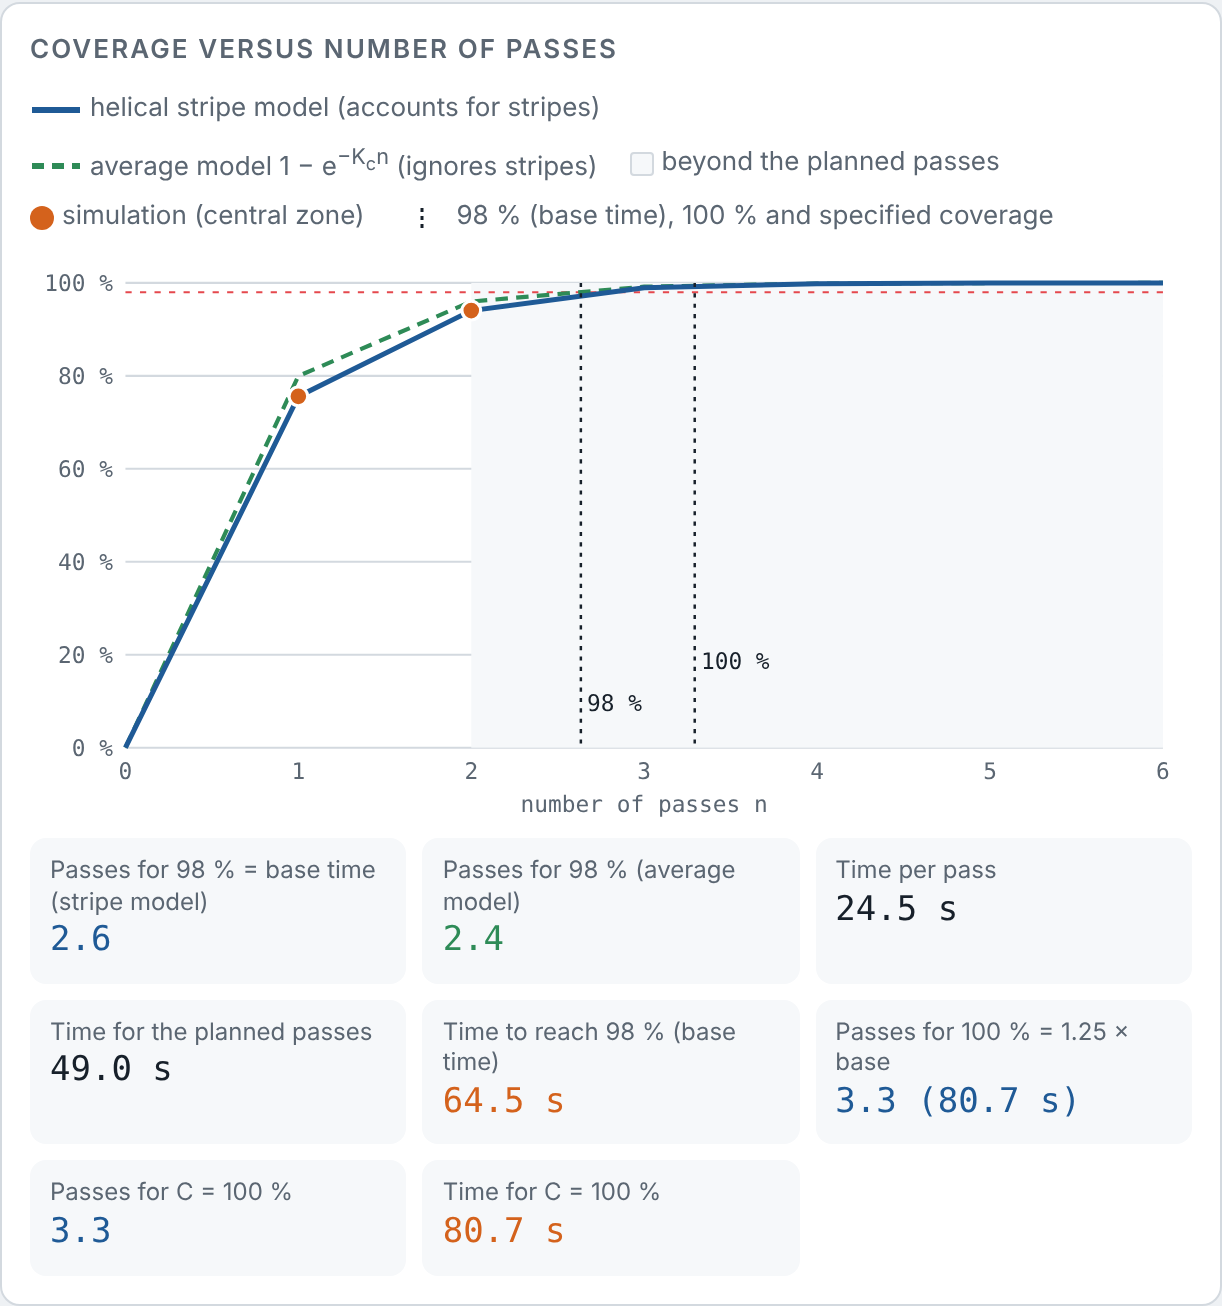
\includegraphics[width=\linewidth]{img/sec3.png}\caption{Coverage versus passes}\end{subfigure}\hfill
\begin{subfigure}{0.49\linewidth}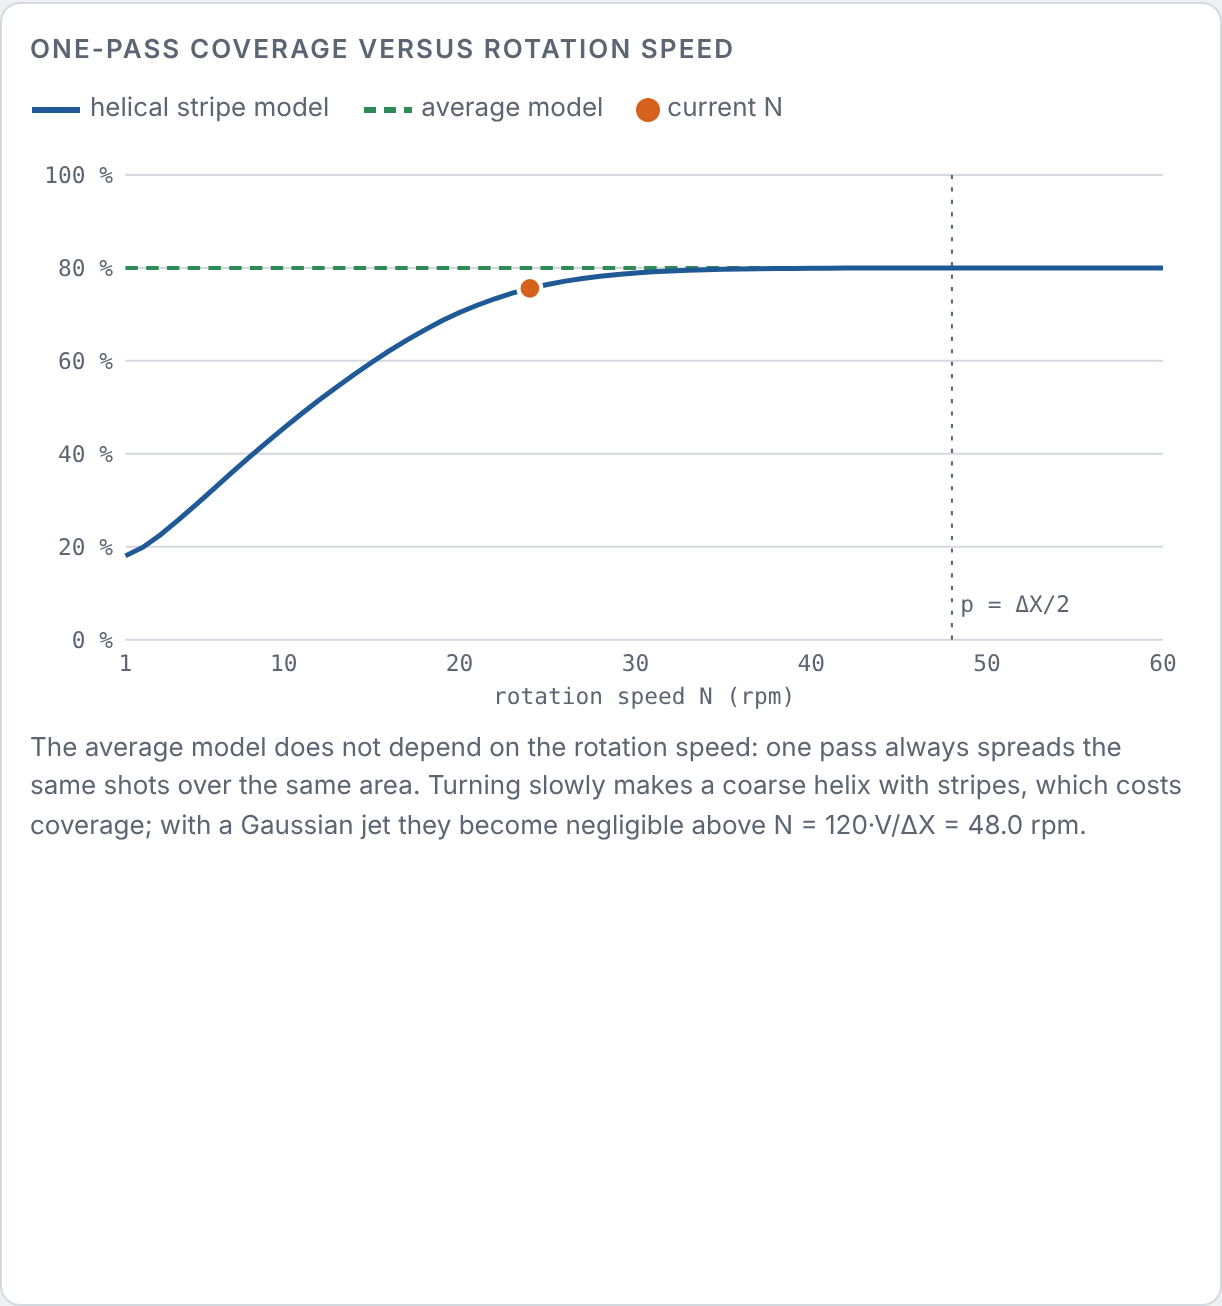
\includegraphics[width=\linewidth]{img/sec4.png}\caption{One-pass coverage versus rotation speed}\end{subfigure}
\caption{Charts with the defaults. Right: the average model is flat, the helical stripe model loses coverage at low speed; the dashed vertical line marks $p=\dX/2$.}
\end{figure}

\section{Algorithm and validation}

\paragraph{Grid.} The unrolled surface ($L\times2\pi R$) is divided into square cells of side
\[
h=\max\Bigl(\sqrt{2\pi RL/250\,000},\ \dX/60,\ \min\bigl(\dX/8,\ p/6,\ 2\pi R/240,\ L/300\bigr)\Bigr),
\]
fine enough to resolve the footprint and the stripes but limited to about 250\,000 cells; the circumferential direction is periodic.

\paragraph{Deposition.} The motion is cut into short segments. When the rotation dominates ($V_s\ge V$), each segment follows the circumference: the impacts are integrated exactly along $s$ with the integral of the cumulative circumferential profile, and averaged over each cell across ($z$). When the traverse dominates, the roles are swapped. The drift across the dominant direction during a segment is limited to half a cell, or 1/40 of the footprint if larger. The 3D view samples the same map, with the shading of a lit cylinder.

\paragraph{Validation.} An independent brute-force calculation in Python (footprint evaluated point by point, small time steps, same pass plan) gives the same mean coverage as the page to within 0.1\,\% for radii from 5 to 200\,mm, uniform, Gaussian and flattened jets, back-and-forth and one-way passes, a jet wider than the cylinder, and with or without the curvature correction (Table~\ref{tab:valid}).

\begin{table}[H]
\centering\small
\caption{Validation of the cylinder simulator: mean coverage in the central zone (\%). Media and jet $\dX=\SI{20}{mm}$ as in the reference case.}
\label{tab:valid}
\resizebox{\linewidth}{!}{\begin{tabular}{@{}lccccc@{}}
\toprule
Case & Page (simulation) & Page (stripe model) & Brute force & Average model\\ \midrule
$R=25$, $L=150$, 24\,rpm, 8\,mm/s, 2 passes & 94.0 & 94.0 & 94.03 & 96.0\\
$R=50$, $L=150$, 20\,rpm, 5\,mm/s, 2 passes & 92.0 & 92.0 & 92.04 & 92.4\\
as first, uniform jet, 1 pass & 80.0 & 79.9 & 79.96 & 80.0\\
$R=40$, 15\,rpm, 6\,mm/s, flattened $p=4$, 3 one-way & 98.2 & 98.2 & 98.16 & 98.2\\
$R=5$, $L=100$, 2\,rpm, 10\,mm/s, 1 pass ($c=68.3\,\%$) & 48.2 & 48.1 & 48.08 & 98.8\\
$R=10$, $L=120$, 30\,rpm, 5\,mm/s, no curvature & 100.0 & 100.0 & 100.0 & 100.0\\
$R=200$, $L=100$, 5\,rpm, 3\,mm/s, 1 pass & 33.5 & 33.5 & 33.48 & 41.5\\ \bottomrule
\end{tabular}}
\end{table}


\section{Things to try}

\begin{center}
\small
\begin{tabular}{@{}lccccl@{}}
\toprule
Change from the defaults & $p$ (mm) & stripes 1 pass & mean $\tau$ (2 passes) & $n_{98}$ & Comment\\ \midrule
none ($N=24$) & 20 & 114\,\% & 94.0\,\% & 2.6 & helix visible\\
$N=48$\,rpm & 10 & 2.8\,\% & 96.0\,\% & 2.4 & stripes gone\\
$N=5$\,rpm & 96 & 650\,\% & 48.1\,\% & 15.5 & coarse helix\\
same direction & 20 & 114\,\% & 95.7\,\% & 2.5 & stacked helices\\
uniform jet & 20 & 0.3\,\% & 96.0\,\% & 2.4 & $\dX/p=1$\\
flattened jet & 20 & 93\,\% & 94.6\,\% & 2.6 & \\
$R=\SI{5}{mm}$ & 20 & 95\,\% & 100\,\% & 0.9 & 31.7\,\% of shots miss\\
$R=\SI{200}{mm}$, $N=5$ & 96 & 763\,\% & 23.2\,\% & 21.4 & large slow drum\\ \bottomrule
\end{tabular}
\end{center}

\begin{trybox}
\begin{itemize}[nosep,leftmargin=*]
\item Use \ui{+1 turn} and watch the unrolled map: each turn adds one tilted band, shifted by the pitch.
\item Compare the two pass sequences with the same number of passes: crossed helices leave a diamond pattern, stacked helices keep their stripes.
\item Choose random phases and press \ui{Restart} several times: with stacked helices the result changes from one draw to the next.
\item Take $R=\SI{5}{mm}$ and switch the curvature off and on: on such a thin part a \SI{20}{mm} jet loses about a third of its shots.
\end{itemize}
\end{trybox}

\section{Assumptions and limits}
Constant rotation and traverse speeds; parallel jet aimed at the axis; the jet keeps firing in the overtravels beyond the ends; dent size independent of the incidence angle; impacts at independent random positions (Poisson), shown through their expectation; no shadowing by shoulders or fillets. The model describes how the surface gets covered, not what happens physically beyond full coverage. It does not replace coverage verification according to the applicable standards (NF~L~06-832, SAE~J2277).

\appendix
\section{Symbols}
\begin{tabular}{@{}ll@{\qquad}ll@{}}
$R$ & cylinder radius & $L$ & cylinder length\\
$N$ & rotation speed (rpm) & $V$ & traverse speed\\
$V_s$ & surface speed & $p$ & helix pitch\\
$\alpha$ & helix angle & $\zeta_\pm$ & helical coordinates\\
$g$, $g_s$ & jet profile, on the surface & $c$ & fraction of shots hitting\\
$K_c$ & mean impacts per point per pass & $h$ & track profile\\
$\lambda$ & expected impacts per point & $t_b$ & base time (98\,\%)\\
$C$ & specified coverage & $\lambda_{100}$ & impacts per point at 100\,\%\\
\end{tabular}

\vfill
\noindent\small Code: MIT licence. Documentation: CC BY 4.0. Related tools: \url{https://rkubler.github.io/shotpeening/}.
\end{document}
